\chapter{Conclusion - Chapter is Work In Progress}
It is time to look back at the work that has been done, to highlight the progress that has been made, but also the shortcomings and gaps that need to be filled by future improvements. We will therefore use this chapter to discuss some of the key points that emerge from this thesis.
 
\section{Intended use of the FuxCP tool}
Throughout this work, it is clear that all the examples provided are fairly short (fourteen bars at most). This is primarily due to Fux himself, as the examples he gives are always of the same shortness, probably for pedagogical purposes. He does not mention this explicitly, but there may also be a practical reason for considering only such short compositions. Indeed, these small compositions can be considered as 'blocks', which can then be arranged to form a whole. The great advantage of this approach is that the countrepoints can be given different species between the blocks, allowing the composition to be constantly renewed.

\begin{figure}[h]
  \centering
  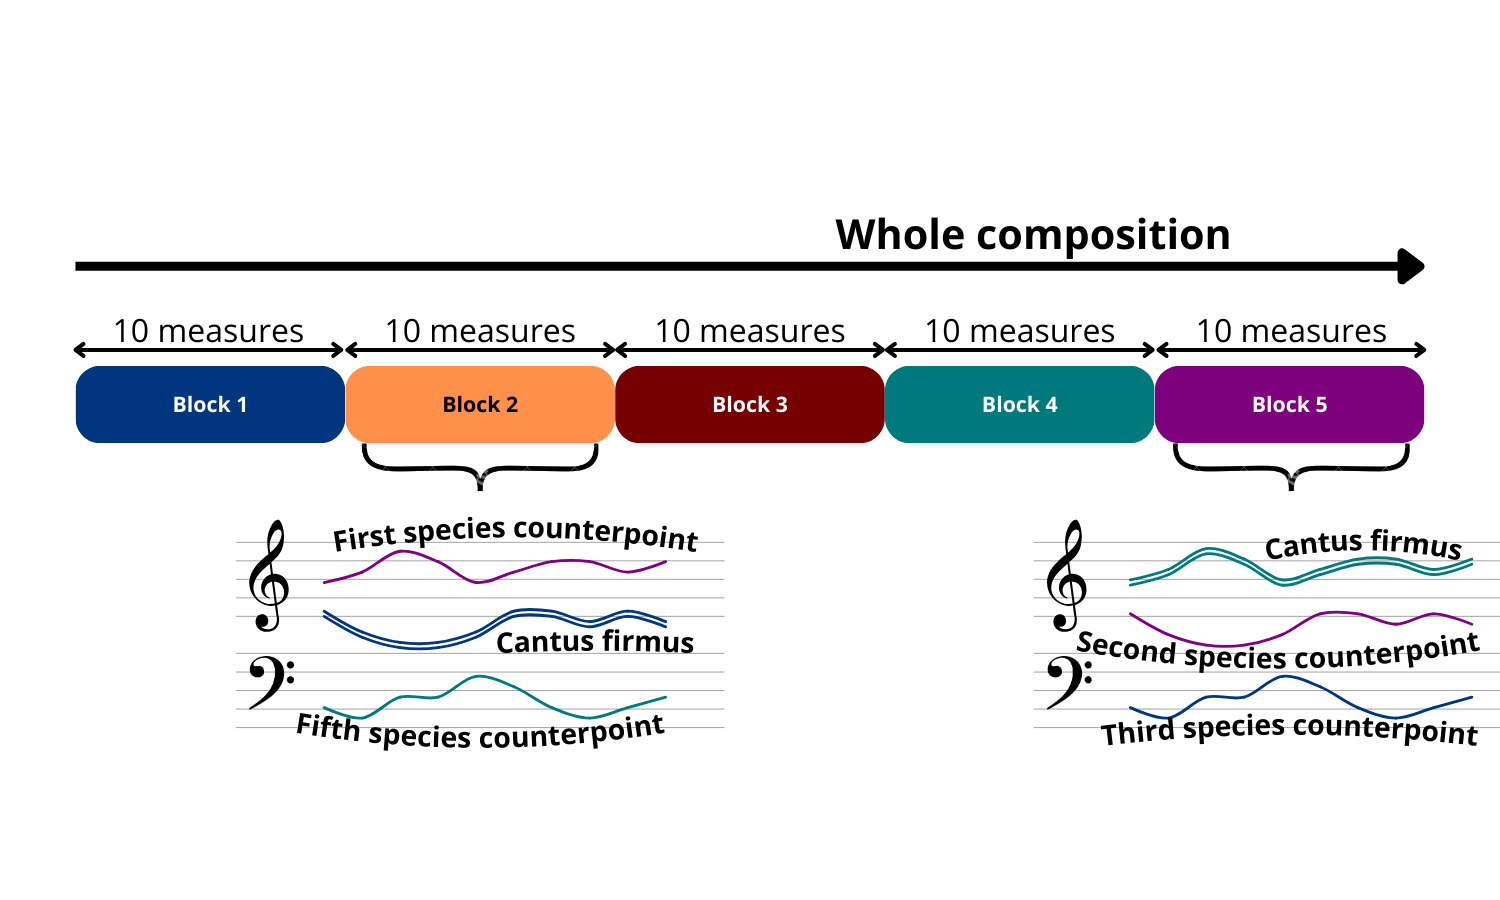
\includegraphics[width=1\textwidth]{Images/composition-in-blocks.png}
  \caption{Example of what of a composition in blocks could look like}
  \label{fig:composition-in-blocks}
\end{figure}

\section{Known issues about the current state of the work} \label{section:known-issues-about-the-current-state-of-the-work}
\begin{itemize}
  \item As mentioned in section \ref{section:time-to-find-a-solution}, some few combinations of species, voice ranges and \textit{cantus firmi} cause the solver to fail to find a solution. The current roundabout way to "solve" this is to... change the voice ranges or some other parameter until a structural solution is found. These cases are relatively rare and do not prevent the use of FuxCP.
  \item If a counterpoint of the fourth species is the lowest stratum, the solver needs more time to find a solution in which all notes are ligated. This is not a problem when combining a fourth species counterpoint with a simple species counterpoint (first or second species), but becomes difficult to handle with more complex species (third or fifth species), as the search time before the solver finds a suitable solution (i.e. with all notes tied) can become very long.
  \item The current heuristics make the solver branch on the lowest stratum array with a "select the values greater than (min+max)/2" policy. For some reason, it always seems to take the lowest value (or close to it), which means that the melody of the voice that is the lowest stratum is really redundant, something that even variety preference doesn't compensate for on complex species, since the time needed to find a good solution (i.e. one where the variety cost is low, which again means that many notes are different) is too high compared to the time needed to find a passable solution.
  
  This leads to a second problem, which is that since the downbeat of the part, which is the lowest layer, always consists of the lowest possible note, the following notes (e.g. in the upbeat) will necessarily be higher. This is because the note in the 2nd, 3rd and 4th bars cannot be the same as the note in the 1st bar, but because the 1st bar is already the lowest possible, the notes in the 2nd, 3rd and 4th bars must be higher. 
  
  As this may be difficult to understand, see Figure \ref{fig:limitation-lowest-array}, which shows that the second species of counterpoint, in the bass, is composed exclusively of upbeat notes that are higher than the downbeat notes. This is a side effect of the heuristic, and a way should be found to resolve it. Note that in this example the problem is solved very quickly (a matter of seconds) because in this setting the other counterpoint is a first species counterpoint (i.e. the setting is not complex, as explained in \ref{section:time-to-find-a-solution}) and the and the solver finds solutions where the upbeat is not always higher than the downbeat very quickly.
\end{itemize}
\begin{figure}[h]
  \centering
  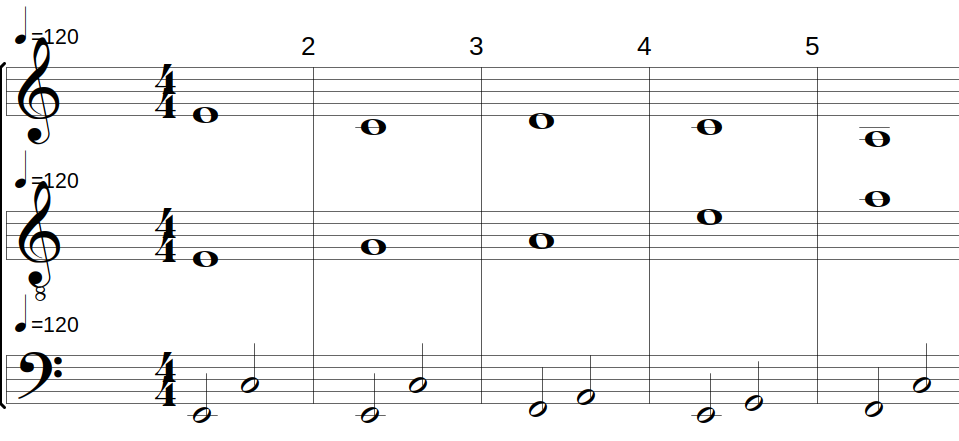
\includegraphics[width=.6\textwidth]{Images/limitation-with-lowest-array.png}
  \caption{Illustration showing the limitation of current heuristics, as the counterpoint of the second species always has a higher upbeat than its downbeat. Note that the composition has been cropped.}
  \label{fig:limitation-lowest-array}
\end{figure}




\section{Future work}
The work towards fully automated counterpoint composition is progressing, but there is still a long way to go before we can claim to have finished the job. There are several ways to improve the current situation for those who want to improve FuxCP. Here are some ideas for improvement:
\begin{enumerate}
  \item \textbf{Solution quality improvements}
  \begin{itemize}
    \item \textit{Finalise the formalisation of \gap} -- The first obvious way to improve the tool is simply to complete the formalisation of Fux's work, which would make it possible to compose in four voices, but also to integrate the additional rules he mentions in his last chapter. This would make it possible to have a complete FuxCP tool, in terms of Fux's rules, and then to supplement Fux's rules with additional rules that could come from any influence. This idea of adding external rules to the Fux rules has already been tested to some extent in the work of T. Wafflard, and the results were more than promising. It is therefore clearly a direction to take in the improvement of the FuxCP tool.
    \item \textit{Relate the notes of the 2nd, 3rd and 4th beats to each other} -- As mentioned in one of the preference ordering experiments (see \ref{subsection:third-experiment-with-costs}), there are no direct constraints between the 2nd, 3rd and 4th beats of each counterpoint. The only way they influence each other is through the transitivity of the constraints: A and B are constrained together, and so are B and C, so A and C are connected in some way. The reason there are no direct constraints is that Fux didn't mention any. Anyway, this leads to some unmelodicity, and it is definitely a good idea to find some rules (e.g. from other authors) that could deal with this unmelodicity. 
    \item \textit{Address any of the current limitations} -- The section \ref{section:known-issues-about-the-current-state-of-the-work} discusses some limitations and issues with the current state of the work. Solving any of them would be an improvement for FuxCP.
  \end{itemize}
  
  
  \item \textbf{Software architecture}
  \begin{itemize}
    \item \textit{Migrate the project to C++} -- Gecode is written in C++, and C++ is a language much better suited to managing implementations like FuxCP. GiL works really well, but has shown its limitations more than once: way too verbose, hard to manage objects (which are useful for designing FuxCP) since using Lisp, and lacking some of Gecode's features. These reasons alone are a huge incentive to migrate the whole implementation to C++. This would make it possible to further improve the implementation with more convenience and efficiency.
    
    Here we repeat the words of T. Wafflard, who had already reached the same conclusion:
    \begin{quotation}
      ``Currently, constraints are added to a species via a long function that dispatches the constraints, rather than via class inheritance. Ideally, object-oriented inheritance
      should be used to represent the different variable arrays and species. All variable arrays (H, M , P , etc.) have something in common, whether in terms of their size rel-
      ative to the cantus firmus, or in terms of the way certain rules are applied. A relatively abstract class should represent this type of array to enable these commonalities to be brought together.

      The same applies to species that share common rules and should have been represented in a class system of their own. It would be logical for species to be children of the first species. Unfortunately, the scope of this work does not allow for a complete overhaul of the architecture. Moreover, in the near future, the entire code may have to be redone in C++ for reasons of performance, features, maintainability, and so on.
      Also, GiL has reached its limits, both in terms of ease of programming and in terms of possibilities. The Lisp language is not designed for writing mathematics, since each operation requires a different function call. Code readability can become complicated because these calls are all represented by parentheses. At the same time, it is not possible with GiL to combine basic mathematical operations to form a larger one. One has to break down each complex operation into simple intermediate basic operations a bit like writing assembly, which is undesirable for larger projects. Not to mention that branch-and-bound, heuristics, and multithreading seem complicated to implement in
      GiL.'' \cite[p.67]{wafflard2023}
      \end{quotation}
  \end{itemize}

  \item \textbf{Solver performance}
  \begin{itemize}
    \item \textit{Bettering the heuristics and reorganising the constraints} -- Obviously, increasing the speed at which the solver finds solutions increases the speed at which the solver finds good solutions. It is therefore crucial to continue working on the heuristics to find better and better solutions. At the same time, once the globality of \gap has been formalised, it might be interesting to rethink the constraints that apply to the composition in an intelligent way, to make the solver's work easier and to have a set of constraints that hold together better.
  \end{itemize}
\end{enumerate}